\documentclass[10pt]{article}
\usepackage[margin=0.5in]{geometry} 
\usepackage{amsmath,amsthm,amssymb, graphicx, multicol, array}

\usepackage[utf8]{inputenc}
\usepackage{graphicx}

\newenvironment{problem}[2][Problem]{\begin{trivlist}
\item[\hskip \labelsep {\bfseries #1}\hskip \labelsep {\bfseries #2.}]}{\end{trivlist}}

\begin{document}
%---------------
%---------------
 \title{Problem Set \# 1 Solutions}
\date{}
\maketitle
 
\begin{problem}{1}
\item
a)\\
For a general wave: Amplitude, mass density, tension, velocity.\\
For periodic waves: wavelength and frequency
\item
b)\\
$A_1 \neq A_2$ - Different because they depend on the initial disturbance or driving oscillation.\\
$\mu_1 = \mu_2$ - It's the same string.\\
$F_1 = F_2$ - Tension is the same if the waves are created without changing the setup.\\
$v_1 = v_2$ - Since, $v = \sqrt{\frac{F}{\mu}}$, the wave speed is the same because density and tension are the same.\\
$f_1 \neq f_2$ - You can drive periodic oscillations with different frequencies on the same string.\\
$\lambda_1 \neq \lambda_2$ - Since wave speed is the same, but frequency can be different, wavelength can also be different.
\item
c)\\
From (b) we saw that wave speed was the same. Since $v = f\lambda$, if the frequencies are the same then lambda must also be the same.
\end{problem}

\begin{problem}{2}
The power in a wave is proportional to the square of the the wave function, so any negative regions of sinusoidal waves will become positive when squared, making the overall power strictly positive.
\end{problem}

\begin{problem}{3}
\item
The tension must be the same across the string segments, others there would be longitudinal motion, which is not possible in the case of strings where we only have transverse motion.
\item
The wave speed depends on tension and density, and we know the density changes. With constant tension, the wave speed must change in the two segments.
\item
If you made periodic waves, the frequency must remain the same across the connection of the segments, otherwise the right most part of segment 1 would separate from the left most part of segment 2.
\item
Since the frequency is constant and the wave speed changes, the wavelength must also change in the two segments for periodic waves.
\item
The amplitude changes because the power has to remain constant. In class we saw that $Power =  \frac{1}{2}\mu v (2\pi f)^2 A^2$ and we can use $v = \sqrt{\frac{F}{\mu}}$ to write $Power = \frac{1}{2} \sqrt{\mu F} (2\pi f)^2 A^2$, meaning that with constant tension and frequency and different density, only amplitude can change to keep power constant.
\end{problem}

\begin{problem}{4}
\item a) The total time is the sum of the individual times for the the wave to move through each segment, $t = L/v$. Replacing $v$ with tension and respective densities and summing gives:
$time = L \sqrt{\mu_1/ F}\left(1 + \sqrt{5} + \sqrt{1/2}\right)$
\item b) You can rearrange the segments as much as you want. Since we add up the individual segment travel times to get total time, each segment time is independent of where it is in the assembly.

\end{problem}

\begin{problem}{5}
A wave is described by the wave function,
\begin{align}
y(x, t) = (8.0mm) sin 2 \pi \left( \frac{x}{32cm} - \frac{t}{0.08s}\right) \nonumber
\end{align}
\item $A = 8.0mm$, $T = 0.08s$, $\lambda=32cm$, the wave moves to the right (positive) because of the minus sign.
\item
b) $v = \lambda f = \lambda / T = (32cm)/(0.08)=4m/s$
\item
c) see below
\item
d) $t=0.40s$, what is the velocity of the string at $x=8cm$?
\begin{align}
\frac{\partial y}{\partial t} = -(8.0mm)\frac{2\pi}{T} cos 2 \pi \left( \frac{x}{32cm} - \frac{t}{0.08s}\right) \nonumber
\end{align}
\begin{align}
\frac{\partial y}{\partial t} = -(8.0mm)\frac{2\pi}{0.4s} cos 2 \pi \left( \frac{8cm}{32cm} - \frac{0.4s}{0.08s}\right) \nonumber
\end{align}
\begin{align}
\frac{\partial y}{\partial t} = -(8.0mm)\frac{2\pi}{0.4s} cos 2 \pi (-4.75)=0\nonumber
\end{align}
\item
e) When $t=0$, what is the velocity of the string at $x=8cm$?
\begin{align}
\frac{\partial y}{\partial t} = -(8.0mm)\frac{2\pi}{0.4s} cos \pi/2 = 0\nonumber
\end{align}
This is unfortunately an accident that both velocities were zero.
\item
f)
\item $Power =  \frac{1}{2}\mu v (2\pi f)^2 A^2$
\item
$Power =  \frac{1}{2} (5.10^{-3}kg)(4 m/s)  (2\pi/.08s)^2 8mm^2 = 3.9 10^{-3} W$

\end{problem}

\begin{figure}[htp]
    \centering
    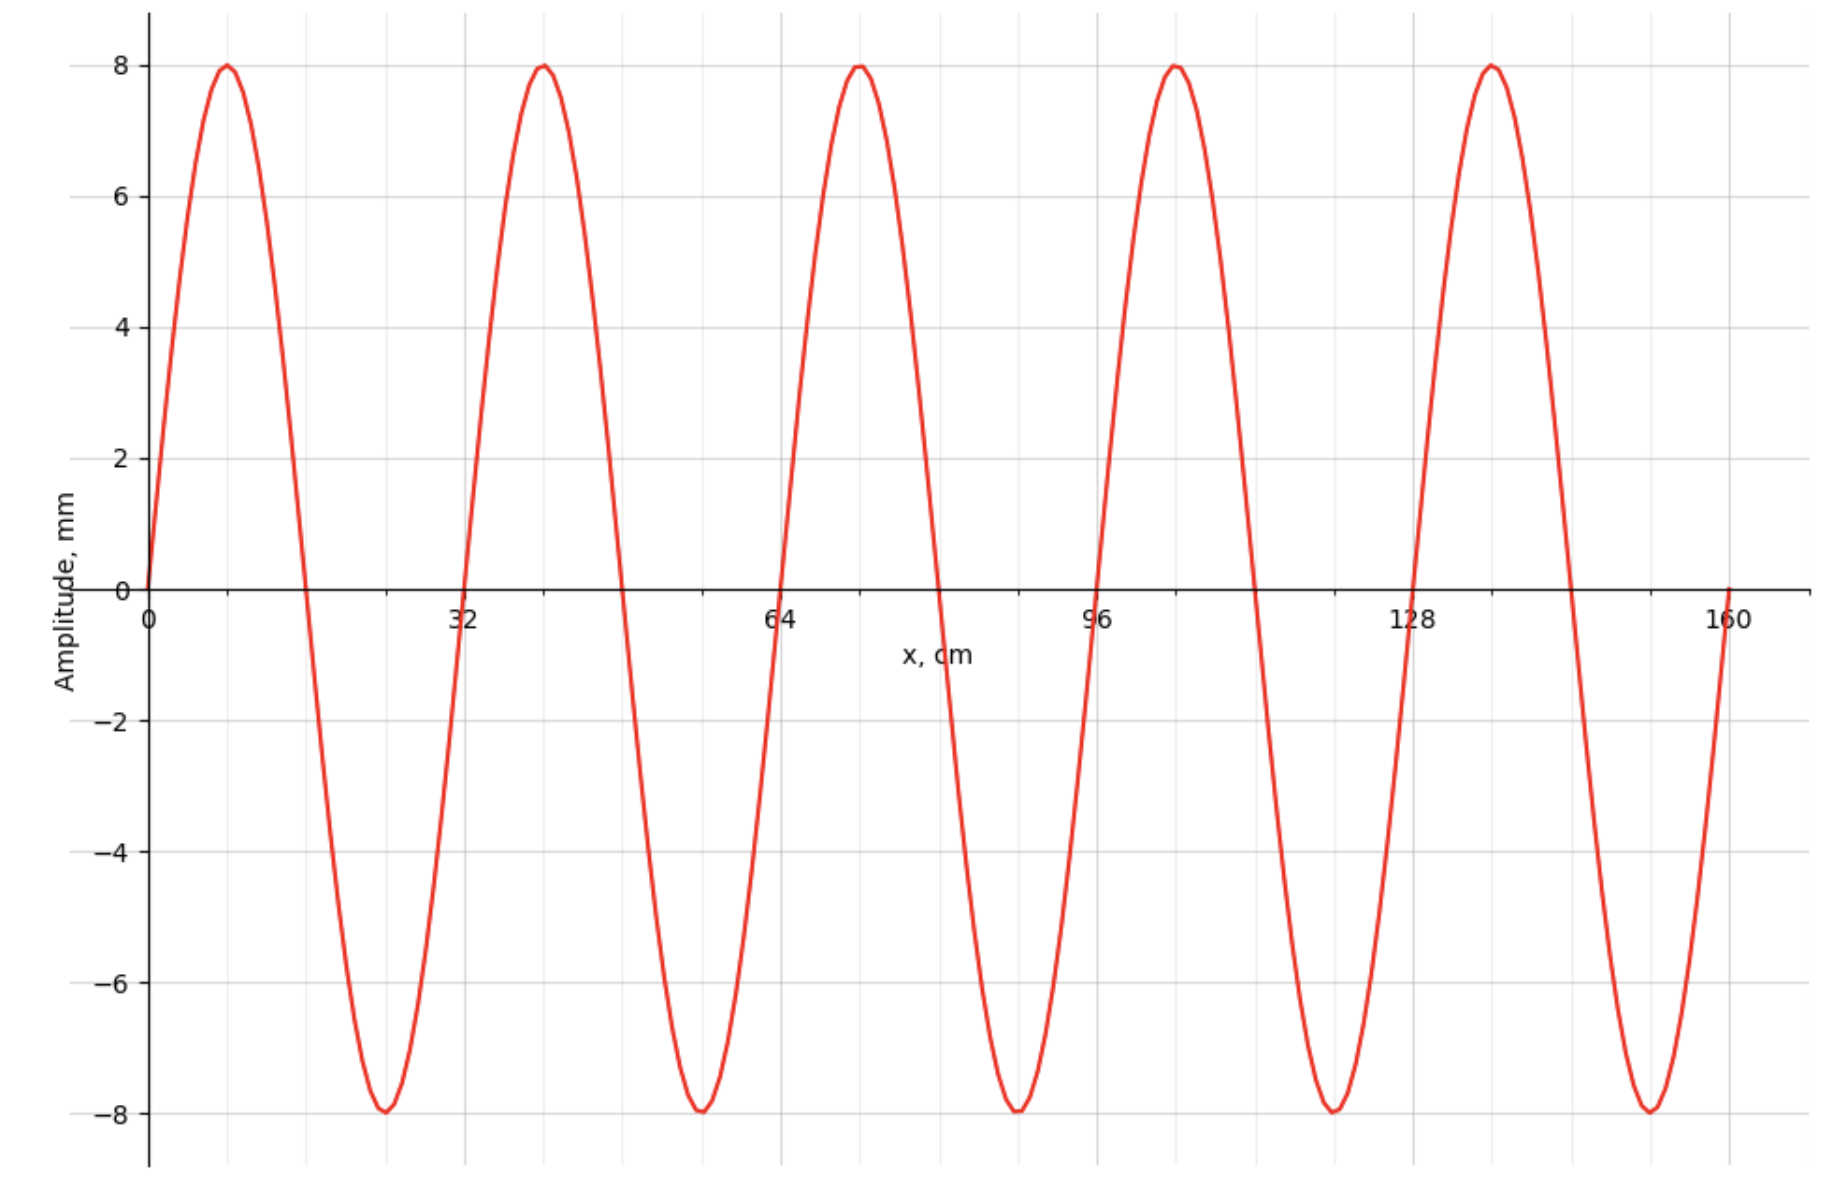
\includegraphics[width=7in]{wavegraph.png}
    \caption{5 (c)}
    \label{fig:Graph of Wave}
\end{figure}


%-------------
%-------------
\end{document}